% (M5-M24) Leader: NCSR "D"
% CeADAR, UPC, ATOS, EVIDEN, FDI, INRIA, ARCADA, use case partners

This section addresses the challenge of estimating the quality of time-series data and introduces a task-agnostic framework for anomaly detection. First, we define the problem and point out the limitations of current methods. Next, we explain our proposed approach, which includes both machine learning and statistical techniques for estimating noise. Finally, we evaluate our framework on the Bitbrain dataset, comparing our results against Bitbrain's own noise detection method, as well as MNE Filtering.

\subsection{Problem Statement}

The quality of time-series data plays a crucial role in the performance of machine learning models, yet existing methods often fail to effectively identify and handle noise in a task-agnostic manner. Traditional data quality estimation techniques are typically tailored to specific datasets, limiting their applicability to a wider range of applications. 

To address these challenges, we propose a task-agnostic framework for time-series data quality estimation. Towards this goal, we propose methods for anomaly and noise detection, which allow us to identify biased, noisy, inconsistent, or otherwise low-quality data, as well as data that may have been maliciously manipulated to contaminate the model during training. Our framework is task-agnostic, meaning it can be applied across different time-series datasets, regardless of the specific task or domain.

As a case study to validate our methods, we use the Bitbrain dataset, which consists of EEG signals collected from a headband across 128 recordings. This headband includes two EEG channels synchronized with medical-grade EEG devices. The signals are annotated by three experts, with each 30-second segment classified into one of five sleep stages: Wake, N1, N2, N3, and REM. These stages correspond to specific brain activity patterns, such as slow eye movements, sleep spindles, and other characteristic waveforms.

% To further validate the robustness of our proposed methods, we explore data augmentation techniques, including adversarial machine learning methods that introduce controlled noise contamination into the dataset.

\subsection{Proposed Methodology}

We propose a task-agnostic framework for time-series data quality estimation, using a combination of machine learning-based and statistical approaches to detect noise and anomalies in data. The techniques used in this framework estimate noise via:

\begin{enumerate}
    \item[(a)] \textbf{Reconstruction error:} unsupervised machine learning using autoencoders, which compress data into a lower-dimensional representation and then reconstruct the original input.
    \vspace{-0.4cm}
    \item[(b)] \textbf{Prediction error:} unsupervised machine learning with transformers, which predict the next sequence of data points.
    \vspace{-0.4cm}
    \item[(c)] \textbf{Attention matrix:} supervised and unsupervised machine learning with transformers and autoencoders, which perform tasks such as classification, reconstruction and prediction.
    \vspace{-0.4cm}
    \item[(d)] \textbf{Statistical function:} statistical methods that detect anomalies by analyzing changes in data characteristics over time.
\end{enumerate}

To apply these techniques, we implement the following 10 methods: LSTM Autoencoder, Convolutional LSTM Autoencoder, Attention-based Autoencoder, Transformer Classifier, Transformer Predictor, Cumulative Sum Control, Page-Hinkley Test, Kullback-Leibler Divergence, Principal Component Analysis and Adaptive Windowing. The last 5 statistical methods are implemented using the \href{https://github.com/IFCA-Advanced-Computing/frouros}{Frouros} framework. Table~\ref{table:framework-summary} summarizes the categorization of each method in the framework across three dimensions: (1) whether the approach is supervised or unsupervised, (2) whether it falls under machine learning or statistical techniques, and (3) how noise is estimated (i.e., reconstruction error, prediction error, attention matrix, or statistical function).

\begin{table}[ht]
    \renewcommand{\arraystretch}{1.5}
    \setlength{\tabcolsep}{12pt}
    \centering
    \caption{Categorization of methods based on noise estimation approach, learning type, and technique.}
    \begin{tabular}{|c|c|c|c|c|}
    \hline
    Approach & \multicolumn{2}{c|}{Machine Learning} & \multicolumn{2}{c|}{Statistical} \\ \cline{2-5} 
             & Unsupervised & Supervised & Unsupervised & Supervised \\ \hline
    Reconstruction Error & \parbox[c][2cm][c]{2.3cm}{\raggedright LSTM-AE\\Conv-LSTM-AE\\Attn-AE} & --- & --- & --- \\ \hline
    Prediction Error     & Predictor & --- & --- & --- \\ \hline
    Attention Matrix     & \parbox[c][1.5cm][c]{2.3cm}{\raggedright Attn-AE\\Predictor} & Classifier & --- & --- \\ \hline
    Statistical Function & --- & --- & \parbox[c][3cm][c]{2.5cm}{\raggedright CUSUM\\PH-Test\\KL-Divergence\\PCA\\ADWIN} & --- \\ \hline
    \end{tabular}
    \label{table:framework-summary}
\end{table}

In our analysis, we chose to estimate noise across 30-second segments of the EEG data, which, in the Bitbrain dataset, corresponds to 7,680 samples. Since each method outputs noise values in different scales, we transform these values into binary based on predefined thresholds per channel to establish a common ground for comparison. To define these thresholds, we need to have a sense of how much noise is typically present in the dataset. For example, in the Bitbrain dataset, which contains brain signals during sleep, we don't expect much noise—typically around 99\% of the data is clean.

To evaluate our noise estimations, we use 2 ground truth methods designed for task-specific noise estimation in EEG signals: MNE Filtering and the original Bitbrain estimation method. MNE Filtering is implemented using the \href{https://mne.tools/stable/index.html}{MNE} library, which provides tools for filtering and analyzing neurophysiological data. We treat Bitbrain's method as a black-box approach, to ensure that our task-agnostic estimations remain unbiased by the specifics of its implementation. Similarly, when using the MNE library, we treat it strictly as a tool, integrating it into our code without really accessing its internal methodology.

\subsection{Machine Learning Approach}
The general concept of using machine learning (ML) for noise estimation revolves around training models to solve specific tasks and then using their outputs during inference to estimate noise. These tasks may vary in nature — ranging from signal reconstruction and prediction to classification — but the core idea is that the model’s performance on these tasks can be used to infer the presence of noise.

To train the models, we split the dataset into training (43 recordings), validation (3 recordings), and testing subsets (10 recordings). Noise estimation is performed using the test dataset. For the training configuration, we set the batch size to 512 and train the models for a maximum of 1000 epochs. To prevent overfitting, we employ early stopping with a patience of 30 epochs, meaning that if the validation loss does not improve for 30 consecutive epochs, training will stop. We set the learning rate to $1e^{-4}$ and use the Adam optimizer to adjust the model weights. Additionally, we implement a \emph{ReduceLROnPlateau} scheduler to dynamically adjust the learning rate based on the validation loss. If the validation loss plateaus, the scheduler reduces the learning rate to help the model continue improving.

To ensure robust model training and reliable outcomes, we rely on data preprocessing techniques. Proper preprocessing standardizes the input data, mitigates inconsistencies, and enhances the model’s ability to learn meaningful representations. In our case, preprocessing involves handling missing or ambiguous data by removing rows containing NaN values, as well as any samples where expert annotators could not agree on the class label (i.e., samples with a label value of 8). Additionally, we apply normalization to assist model training by making the data more uniform. Due to the low variability and the presence of extreme outliers in the EEG signals, we adopt a robust normalization approach. Instead of using the mean and standard deviation, which are sensitive to outliers, we use the median and interquartile range (IQR). We scale the data based on statistics computed across the entire dataset, rather than on a per-batch basis, since the statistics remain consistent across the full dataset.

\begin{equation}
    x_{\text{norm}} = \frac{x - \text{median}(x)}{\text{IQR}(x)} \label{eq:robust_norm}
\end{equation}

where $x$ represents the values of a particular feature, $\text{median}(x)$ is the median value of the feature, and $\text{IQR}(x)$ is the interquartile range, which measures the spread of the middle 50\% of the data. We use the median as a measure of central tendency because it is robust against extreme values, making it a more reliable indicator for our dataset, which exhibits low variability and where even small differences matter. Additionally, we use the interquartile range $\text{IQR} = Q_3 - Q_1$ to reduce the influence of outliers by focusing on the range within which the central portion of the data lies. This approach ensures that our normalization process allows the model to learn from the true patterns in the dataset.

To process the input data, we split each 30-second segment of EEG data (7,680 samples) into 32 smaller chunks, resulting in 240 sequences per segment. Each sequence has a length of 240 time steps, with 2 features corresponding to the EEG channels. This structure allows the model to focus on both the short- and long-term temporal dependencies within the data. Additionally, we notice that our dataset tends to overfit with more complex models due to its low variability and extreme outliers. To mitigate this, we use simple architectures with only a few layers, e.g. a single attention layer in the attention-based models. This approach avoids unnecessary complexity, ensuring more stable training and better generalization on the data.

For all machine learning methods, we need to establish a common standard to determine what is considered noise and what is not. As the models output different value ranges, we need a policy to classify these outputs into binary values that indicate noise presence or absence. One such approach involves defining thresholds that act as a boundary between noise and clean data. For these methods, we define thresholds based on the 99th percentile of noise values for each channel. Values above the thresholds are set to 1 (indicating noise), while those below are set to 0 (indicating no noise).

Noise estimation within this machine learning approach can be divided into two categories: label-based and label-free:

\begin{itemize}
    \item The label-based approach involves training classifier models on labeled data to learn how to assign class labels to signals. The \emph{Transformer Classifier}, trained to classify signals into sleep stages, belongs to this category. The idea is to use the model’s attention matrix, which highlights the importance of different time steps in data, to infer the presence of noise. Higher attention values correspond to segments of data that are likely noisy, whereas lower attention values indicate cleaner segments of data.
    \vspace{-0.2cm}
    \item The label-free approach does not rely on labeled data for training. Instead, it focuses on unsupervised techniques to estimate noise based on the characteristics of the signal itself. In this category, we use models like autoencoders and transformers that learn to reconstruct and predict signals respectively. The three \emph{Autoencoders} focus on reconstructing the input data, and noise is identified through the reconstruction error — the larger the error, the more likely the segment is noisy. On the other hand, the \emph{Transformer Predictor} learns to predict the next sequence of data points, and noise is identified through the prediction error. Additionally, both the \emph{Attention-based Autoencoder} and \emph{Transformer Predictor} can estimate noise using their attention matrices. In these models, higher attention values indicate segments of data that are more likely to be noisy, while lower attention values correspond to cleaner segments.
\end{itemize}

\subsubsection{LSTM Autoencoder}

We implement an \emph{LSTM-based Autoencoder} that uses Long Short-Term Memory (LSTM) layers to reconstruct EEG signals from a lower-dimensional latent representation. The key idea behind this autoencoding approach is to compress the input signal while preserving the essential features, then reconstruct it from the compressed representation. The LSTM layers in the encoder are designed to capture the temporal patterns and dependencies inherent in the EEG signals. These temporal dependencies are crucial for accurately modeling EEG data, which often exhibits long-range correlations over time. The decoder, in turn, reconstructs the original signal from this latent representation, hoping that only non-noisy information is preserved during compression.

The encoder processes each sequence in the data and compresses it into a latent representation of size (1, 8), where the first dimension represents a single compressed time step, and the second dimension represents 8 learned features. The decoder then takes this compressed representation and attempts to reconstruct the original signal, capturing both trends and amplitudes.

To balance the models' focus on both the amplitude and trends of the EEG signals, we define a custom loss function, called \emph{BlendedLoss}. This function combines the median and mean of the powered absolute differences between the predicted ($\hat{x}$) and target values ($x$):
%
\begin{equation}
\text{Loss} = (1 - \text{blend}) \cdot \text{median}(\lvert \hat{x} - x \rvert^p) + \text{blend} \cdot \text{mean}(\lvert \hat{x} - x \rvert^p)
\label{eq:blended_loss}
\end{equation}
%
where $p$ is the power parameter that controls the sensitivity of the loss to the differences, $x$ is the original signal, and $\hat{x}$ is the reconstructed signal. The blend factor controls the trade-off between learning the overall trends (via the median) and capturing the amplitude (via the mean). We experiment with different blend values (0.1 and 0.8) to observe how this affects the model’s performance in reconstructing the signals.

The \emph{LSTM Autoencoder} estimates noise by measuring the reconstruction error between the original and the reconstructed signal. During training, the model learns to compress and then reconstruct the input signal with minimal error. The goal is for the model to capture the common patterns and trends in the data, such as periodic fluctuations or typical signal behavior. When the model encounters unusual spikes, often caused by noise, it struggles to reconstruct them because they don't fit the typical patterns it has learned. As a result, the reconstruction error for these segments will be larger, indicating noise.

\subsubsection{Convolutional LSTM Autoencoder}

We implement a \emph{ConvLSTM-based Autoencoder} that combines convolutional and LSTM layers to reconstruct EEG signals from a lower-dimensional latent representation. The convolutional layers capture local features in the data, while the LSTM layers capture long-range temporal dependencies. This hybrid architecture is designed to effectively process spatiotemporal data like EEG signals, which contain both spatial (local) and temporal (long-range) patterns.

We use the same \emph{BlendedLoss} function, as defined in Equation~\ref{eq:blended_loss}, to balance the reconstruction of amplitude and trends. Similar to the LSTM approach, noise is estimated through the reconstruction error.

\subsubsection{Attention-based Autoencoder}

We implement an \emph{Attention-based Autoencoder} that combines convolutional layers with a multi-head attention mechanism to reconstruct EEG signals from a lower-dimensional latent representation. The convolutional layers help extract spatial features from the input data, while the attention mechanism is particularly effective in modeling temporal dependencies. This allows the model to focus on important time steps and capture long-term patterns, without the need for recurrent layers like LSTM. The key innovation of this hybrid model lies in the use of multi-head attention, which enables the model to focus on different parts of the input sequence simultaneously. The attention mechanism computes a weighted sum of the input features, with the weights learned during training. This allows the model to prioritize certain features and temporal patterns over others, making it particularly effective for detecting noise or anomalies that deviate from typical signal behavior.

We use the same \emph{BlendedLoss} function, as defined in Equation~\ref{eq:blended_loss}, to balance the reconstruction of amplitude and trends. Regarding noise estimation, we adopt two strategies:

\begin{itemize}
    \item The first strategy defines noise as the reconstruction error, similar to the other two autoencoders.
    \vspace{-0.5cm}
    \item The second strategy defines noise based on the attention weights in the attention matrix. Attention mechanisms allow the model to assign varying levels of importance (i.e., attention weights) to different parts of the input sequence. The key idea is that the attention mechanism can distinguish between relevant and irrelevant time steps by analyzing how much focus the model places on them during the encoding and decoding process. When a time step receives a low attention weight, it suggests that the information at that moment is likely noisy and, therefore, unimportant for the reconstruction task.
\end{itemize}

\subsubsection{Transformer Predictor}

We implement a \emph{Transformer Predictor }that uses multi-head attention for time-series forecasting. This model consists of a sequence-to-sequence architecture, with multi-head attention layers in both the encoder and decoder components. The encoder captures temporal dependencies in the input sequence, while the decoder predicts the next sequence based on these encoded features. The attention mechanism enables the model to focus on relevant time steps, improving its ability to capture long-term dependencies and trends.

To train the model, we use the \emph{BlendedLoss} function, as defined in Equation~\ref{eq:blended_loss}, to balance the reconstruction of amplitude and trends.

The \emph{Transformer Predictor} estimates noise based on two distinct strategies: prediction error and attention weights:
\begin{itemize}
    \item The first strategy, prediction error, focuses on the difference between the model's predicted output and the actual observed values. When the model predicts the next time step in the sequence, a large difference between the predicted and actual values suggests that the input data may be noisy. This is because the Transformer model is designed to learn patterns and trends in the data, and noise, being irregular and unpredictable, disrupts this learning process. As a result, larger prediction errors typically correspond to noisy data, which the model struggles to predict accurately.
    \vspace{-0.2cm}
    \item The second strategy involves the attention weights, derived from the model’s attention mechanism. Similar to the \emph{Attention-based Autoencoder}, the \emph{Transformer Predictor} uses attention to focus on different parts of the input sequence. Noisy segments make it harder for the model to detect consistent patterns and, as a result, tend to receive lower attention weights. On the other hand, time steps that align well with the learned patterns and trends in the sequence typically receive higher attention values.
\end{itemize}

\subsubsection{Transformer Classifier}

We implement a \emph{Transformer Classifier} that uses a multi-head attention to classify sleep stages from EEG signals. The model architecture includes both an encoder and a decoder, with multi-head attention layers in each component to capture temporal dependencies and refine learned features across the input sequence. The encoder captures complex relationships in the input data, while the decoder further processes these features for classification. The attention mechanism enables the model to focus on key time steps in the sequence, helping it identify the most relevant temporal information for predicting sleep stages. Finally, a feedforward classifier layer produces the predicted sleep stages based on the features processed by the encoder and decoder.

To train the model, we use Cross-Entropy loss, which measures the dissimilarity between the predicted probability distribution and the true distribution. This loss function is commonly used for classification problems to penalize the model based on how confident and accurate its predictions are. Given that the dataset is quite imbalanced, with class frequencies reflected by the weights as shown in Table \ref{tab:class_freqs_weights}, we employ a weighted version of the Cross-Entropy loss (see: Equation~\ref{eq:weighted_cross_entropy_loss}). This approach adjusts the influence of each class in the loss calculation, helping the model learn across all class distributions, regardless of their prevalence in the dataset.

\begin{equation}
    \text{Loss} = -\sum_{i=1}^{N} w_{y_i} \cdot \log(p_{y_i})
    \label{eq:weighted_cross_entropy_loss}
\end{equation}

where \(N\) is the total number of samples, \(y_i\) represents the true class label for the \(i\)-th sample, \(p_{y_i}\) is the predicted probability for the true class, and \(w_{y_i}\) is the weight assigned to the class \(y_i\).

\begin{table}[h!]
    \centering
    \caption{Class frequencies and weights used in weighted cross-entropy loss.}
    \begin{tabular}{c|c|c}
    Class & Freqs (\%) & Weights \\
    \hline
    0 & 14.11 & 0.12 \\
    1 & 4.45  & 0.39 \\
    2 & 62.16 & 0.03 \\
    3 & 4.96  & 0.35 \\
    4 & 14.36 & 0.12 \\
    \end{tabular}
    \label{tab:class_freqs_weights}
\end{table}

The \emph{Transformer Classifier} estimates noise based on the attention weights in the attention matrix, similar to the approach used in the attention-based autoencoder. The attention mechanism in the Transformer model assigns varying levels of importance to different time steps in the input sequence. By analyzing the attention weights, we can identify time steps that the model considers noisy, as these time steps receive lower attention weights. The rationale behind this is that the classifier makes strong, confident predictions when the data is clean and well-defined. Noise, by nature, does not fit well into any particular class, and the model finds it harder to assign a clear class label to noisy samples.

\subsection{Statistical Approach}

In addition to machine learning-based methods, statistical techniques offer a robust alternative for detecting noise in time-series data and are widely used. These methods focus on analyzing changes in the statistical properties of the data over time, which can help identify deviations from expected patterns.

Unlike machine learning methods, no normalization is applied to the data, as statistical methods require the raw data to function properly. This ensures that the characteristics of the original signal are preserved, which is crucial for accurate anomaly detection.

In terms of noise thresholding, the Frouros-based methods inherently provide binary outputs based on internal thresholds. These thresholds are designed to classify data as noisy or clean. To handle cases where sample aggregation results in float values, we apply the same noise thresholding method—using the 99th percentile, as in the machine learning-based methods—to convert these results into binary form.

To ensure consistency across all methods and enable meaningful comparisons, the same test recordings used for machine learning-based noise estimation are also applied to the statistical methods.

\subsubsection{Cumulative Sum Control Chart}
Cumulative Sum Control Chart (CUSUM) is a sequential analysis technique commonly used in statistical quality control to monitor change detection \cite{basseville1993detection} by identifying moments when the probability distribution of a stochastic process or time series shifts. Unlike approaches that independently analyze measurements at specified times, CUSUM accumulates information from both current and past samples \cite{ncss2024}. Thanks to this cumulative property, CUSUM proves to be more efficient \cite{nelson1984shewhart} compared to simpler methods such as Shewhart charts \cite{koshti2011cusum}.
CUSUM is represented through the following equation:

\begin{equation}
S_m = \sum_{i=1}^{m} (\tilde{x}_i - \hat{\mu}_0) \quad \text{or} \quad S'_m = \frac{1}{\sigma_{\tilde{x}}} \sum_{i=1}^{m} (\tilde{x}_i - \hat{\mu}_0),
\end{equation}
where: $m$ is the sample number, $\hat{\mu}_0$ is the estimated in-control mean, and $\sigma_{\tilde{x}}$ is the known or estimated standard deviation of the sample means.

In the context of MANOLO, CUSUM is applied due to its capability to detect abrupt changes. By continuously monitoring cumulative deviations from the baseline, CUSUM facilitates rapid detection of this kind of changes.
These properties make CUSUM a strong candidate for noise detection tasks, where, according to the literature, it has shown highly promising results \cite{artyushenko2021modeling}, \cite{volovach2021detection}, \cite{tam2009theoretical}, \cite{yi2021adaptive}.

\subsubsection{Page-Hinkley Test}
The Page-Hinkley Test is a sequential analysis technique used to detect abrupt changes \cite{sebastiao2017supporting} in the mean value of a signal or data stream over time, which may indicate noise or data drift. Additionally, the Page-Hinkley Test is used to monitor the performance of industrial processes \cite{mouss2004test} or assess the efficiency of learning models \cite{ali2023understanding}.

When applying the algorithm, an initial threshold value must be defined, which serves as a reference point. If a change in the mean exceeds this threshold, the change is considered significant. Furthermore, a decision function must be defined, which applies the Page-Hinkley technique by evaluating the data and returning 1 if a change is detected, and 0 if no change is detected.

The Page-Hinkley Test is beneficial for anomalies related to gradual shifts since it accumulates evidence over time, making it robust for detecting slower, cumulative shifts rather than just abrupt changes.

\subsubsection{Kullback-Leibler Divergence}

Kullback-Leibler Divergence (KLD), also known as relative entropy or l-divergence, quantifies the proximity of two probability distributions \cite{joyce2011kullback}. It measures, in bits, how close a probability distribution \( p \) is to a model distribution \( q \) \cite{vanerven2014renyi}, and is defined as:

\begin{equation}
D_{\text{KL}}(p \parallel q) = \sum_i p_i \log_2 \left( \frac{p_i}{q_i} \right)
\end{equation}

where \( p_i \) and \( q_i \) represent the probabilities of each outcome in the distributions \( p \) and \( q \), respectively. The KLD is not symmetric, meaning \( D_{\text{KL}}(p \parallel q) \neq D_{\text{KL}}(q \parallel p) \). The divergence \( D_{\text{KL}}(p \parallel q) \) is zero only when the distributions \( p \) and \( q \) are identical. In other words, this equation represents the average number of extra bits needed to encode samples from distribution \( p \) using an optimal code for distribution \( q \). 

To implement KLD, the data gets divided into consecutive windows. The probability distribution of each window is then estimated, and the KLD between successive windows is computed. If the resulting divergence exceeds a predefined threshold, drift is detected.

In general, KLD is widely used in statistics and pattern recognition, but it also finds applications in speech and image recognition \cite{hershey2007approximating}.

\subsubsection{Principal Component Analysis}

Principal Component Analysis (PCA) is a linear dimensionality reduction technique. It analyzes a data table where observations are described by quantitative dependent inter-correlated variables. With PCA, the important information is extracted from the table and represented in a new set of orthogonal variables, called principal components \cite{bro2014principal}. The similarity patterns of the observations and the variables can then be depicted as points on maps \cite{abdi2010principal}.

PCA is frequently used when a large number of variables have a high degree of correlation with one another, and it is preferable to reduce them to an independent set. Specifically, the variable created as a linear combination of the original variables that accounts for the greatest amount of variance is the first principal component of a set of p variables. After the effect of the first component is eliminated, the second principal component explains the greatest amount of the variance in what remains, and the process can continue through p iterations until all of the variance is explained \cite{jolliffe2016principal}, \cite{shao2014prototype}.

\subsubsection{Adaptive Windowing}

Adaptive Windowing (ADWIN) is a technique that allows for handling concept drift and distribution changes when learning from data sequences that may change over time \cite{bifet2007learning}, \cite{sun2016online}.

ADWIN maintains a variable-length window of recent data points, ensuring that the data distribution remains stable. To detect any changes, this window is subdivided into two sub-windows ($W_0$ and $W_1$). To determine whether a change has occurred, ADWIN compares the averages of $W_0$ and $W_1$. If the equality of the distributions is no longer maintained, concept drift is detected, and $W_0$ is replaced by $W_1$, with a new $W_1$ initialized.

ADWIN uses a significance value \(\delta \in (0,1)\) to assess whether the two sub-windows correspond to the same distribution. If the absolute difference between the means of $W_0$ and $W_1$ exceeds a predefined threshold, an alarm is triggered. 

ADWIN is particularly effective for detecting both sudden and gradual changes in data streams due to its dynamic adjustment of the window size. Additionally, ADWIN is well-suited for cases that often exhibit unpredictable shifts. Its ability to adaptively resize the window makes it ideal for handling such changes without relying on predefined parameters.

\subsection{Evaluation and Results}

To evaluate the effectiveness of the task-agnostic framework, we use two ground-truth methods, both designed for task-specific noise estimation in EEG signals: A) The original estimation method used by Bitbrain, the headband manufacturer B) MNE Filtering.

\subsubsection{Bitbrain Method}
One of the main concerns when dealing with electroencephalographic signals (EEG) is assuring that clean data with a high signal to noise ratio is recorded. The EEG signal amplitude is in the microvolts range, and it is easily contaminated with noise, known as artifacts, which need to be filtered from the neural processes to keep the valuable information needed for different applications. 

In this domain, an artifact is denoted as any component of the EEG signal that is not directly produced by human brain activity, making the system register noise that contaminates the neural EEG data.  
The ability to recognize these artifacts is the first step in removing them. EEG artifacts can be classified depending on their origin, which can be physiological or external to the human body (technical/non-physiological).  

The Bitbrain team develops task-specific algorithms to automatically estimate noise and evaluate the overall quality of EEG signals, identifying the artifacts present in recordings made using their wearable textile headband. 

These algorithms detect several artifacts of different origin, including: 
\begin{itemize}
    \item High amplitude artifacts that may be due to: \begin{itemize}
        \item Temporary failures in contact between the EEG sensor and the scalp produced by touching the sensor or by spontaneous changes in electrode-skin contact. 
        \item Movement of the cables connecting the electrodes and the amplification system. 
    \end{itemize}
    \vspace{-0.2cm}
    \item High frequency noise (30-45 Hz) that may originate from: \begin{itemize}
        \item Electrical activity produced by the muscles when they are contracted. This activity can be measured, and the resulting signal is called electromyography (EMG). Typical effects are muscle tension in the jaw or forehead, that can take place when clenching or frowning, respectively. 
        \item AC electrical and electromagnetic interferences that may arise due to insufficient lack of wire shielding.
        \item Poor electrode-skin contact. 
    \end{itemize}
    \vspace{-0.2cm}
    \item Low frequency noise (0.2-4 Hz) mainly due to: \begin{itemize}
        \item Perspiration originated from small drops of sweat produced by the skin glands, which cause changes in the electrical baseline of the electrodes. In case of intense perspiration, it could even create shorts between electrodes. 
    \end{itemize}
    \vspace{-0.2cm}
    \item Empty segments because of Bluetooth connection loss. 
    \vspace{-0.2cm}
    \item Flat line segments mainly caused by instrumental error where contact between electrodes and skin is lost. 
\end{itemize}
\vspace{+0.9cm}
\begin{figure}[ht]
    \vskip -0.2in 
    \centering
    \caption[Examples of temporal visualization of EEG signals with labelling]{Examples of the temporal visualization of EEG signals together with the labelling of noisy segments (shading). It can be seen which areas of the signal have been identified as artifacts, as well as by which detectors. (Image 1-3: Pink - Low frequency noise (sweat); Brown: High frequency noise (muscle tension). Image 4: Green – High frequency noise; Orange: High amplitude noise).}
    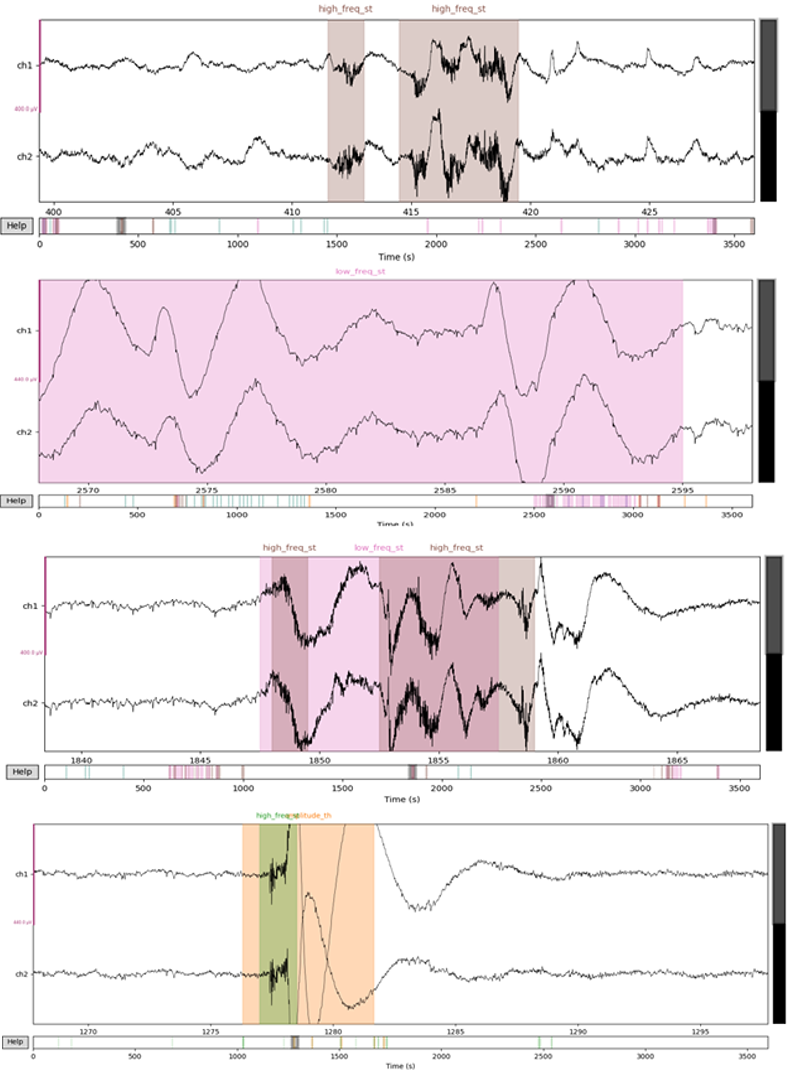
\includegraphics[width=0.6\columnwidth]{fig_dataquality/bitbrain_eeg_and_noise_labels.PNG}
    \label{fig:bitbrain_eeg_noise}
    \vskip -0.0in 
\end{figure}

Prior to applying these algorithms, a band-pass filter is applied to the EEG in the range 0.2-45 Hz. Below, the development of the artifact detectors is discussed in more detail: 
\begin{itemize}
    \item \textbf{High amplitude artifacts:} This method is based on a static amplitude threshold, specified in microvolts. A window is then selected around any point that exceeds the threshold. 
    \vspace{-0.2cm}
    \item \textbf{High frequency noise:} The power in the 30-45Hz power range is estimated using signal windows. Basically, to label a zone as artifactual, the power in the mentioned range must exceed a threshold, which is fixed in a logarithmic scale. 
    \vspace{-0.2cm}
    \item \textbf{Low frequency noise:} The power is estimated in the 0.2-4Hz power range using signal windows. The method applied to recognize an area as an artifact is the same as for high frequency noise. 
    \vspace{-0.2cm}
    \item \textbf{Flat line segments:} This detector identifies time windows where the amplitude does not exceed a very small threshold, close to zero. 
\end{itemize}
All default thresholds were selected based on a statistical analysis of more than 150 EEG sleep recordings. 

The output of the above algorithms provides binary masks that locate and identify noise-contaminated signal segments and their possible source. This automatically generated information can be very valuable for the experimenter, since it is resource-intensive to manually inspect a sleep recording that can last approximately eight hours. 

Within Manolo's Use Case 3, Bitbrain is designing a closed-loop auditory stimulation system during sleep, which will integrate and validate the technology developed throughout the project. The first task performed by the system is the real-time characterization of sleep stages. This is accomplished by an automatic sleep scoring algorithm, consisting of a deep neural network (DNN) that is being trained with the sleep datasets recorded using the wearable device.  

Therefore, the artifact masks generated for this purpose contain an estimate every 30 seconds. In this case, the thresholds of the different detectors were estimated empirically. They were established with the aim of optimizing the artifact removal to maximize data analysis while minimizing the amount of discarded data. By this means, only those artifacts that negatively impact the performance of the model are detected and eliminated.

Table~\ref{tab2} presents the number of artifacts identified by Bitbrain’s method across the ten recordings used for evaluating the task-agnostic framework. It provides the total count of 30-second segments in which at least one artifact was detected for each recording, with results reported separately for each EEG channel (designated as HB1 and HB2).

\begin{table}[htbp]
\caption{Number of segments containing artifacts in the test recordings identified by Bitbrain’s method}
    \centering
    \renewcommand{\arraystretch}{1.3} % Adjust row height
    \begin{tabular}{|c|c|c|c|c|c|c|c|c|c|c|}
        \hline
        \textbf{Recording} & \textbf{1} & \textbf{2} & \textbf{3} & \textbf{4} & \textbf{5} & \textbf{6} & \textbf{7} & \textbf{8} & \textbf{9} & \textbf{10} \\
        \hline
        HB1 & 9 & 57 & 0 & 1 & 27 & 0 & 0 & 1 & 1 & 0 \\
        \hline
        HB2 & 9 & 56 & 0 & 0 & 26 & 151 & 0 & 1 & 1 & 0 \\
        \hline
    \end{tabular}
    \label{tab2}
\end{table}

The table shows that in three out of the ten recordings (3, 7, and 10), neither channel detects any artifacts. In three other recordings (4, 8, and 9), only one segment is found to be contaminated with noise by both channels, except in recording 4, where noise is detected solely by the HB1 channel. In recordings 1 and 2, noisy segments are almost unanimously identified by both channels. Additionally, in recording 6, only the HB2 channel detects noise in several segments, suggesting a potential issue with that particular sensor.

Table~\ref{tab3} presents the Precision and Recall metrics, for the evaluated methods across the seven test recordings (1, 2, 4, 5, 6, 8, and 9) where an artifact was detected by the Bitbrain's method. All values are expressed as percentages.

The Precision metric denotes the percentage of actual segments identified as having artifacts relative to the total segments predicted to contain artifacts. However, this metric fails to convey information regarding missed artifacts---specifically, those not identified by the anomaly detection methodologies. This aspect is quantified through the Recall metric, which indicates the ratio of segments predicted to have artifacts against the total number of actual segments containing artifacts. For instance, the PCA method exhibits a precision of 100\% from the data obtained during the HB1 test recording 1, yet it only achieves a recall of 11.11\%. This discrepancy arises because the PCA method successfully detected a singular artifact characterized by noise, deemed a noisy artifact; thus, the precision remains at 100\%. However, it failed to identify the additional eight noisy segments (refer to Table~\ref{tab2}), resulting in a significantly reduced recall of approximately 11\%. Instances where there are empty cells signify scenarios where the respective method did not identify any artifacts. Consequently, precision cannot be ascertained, and recall is recorded as 0\%.

In this application, our primary objective is to identify as many segments as possible that contain artifacts while allowing for some tolerance regarding detecting noisy segments. The principal aim should be to reduce the number of instances requiring the application of reliable yet non-automated anomaly detection methods. Consequently, the key performance metric to prioritize is Recall.

From the results presented in Table~\ref{tab3}, we conclude that all considered methods exhibited suboptimal performance. However, the PCA demonstrated relatively high recall values in two recordings. One plausible explanation for this observation could be the selected time-window of 30 seconds that defines the examined segment. The efficacy of anomaly detection methods in time series analysis may be significantly influenced by the length of the time series, as supported by existing literature \cite{Lee_2021}.

\begin{table*}[btp]
\centering
\caption{Precision/Recall of the task-agnostic methods with respect to the Bitbrain's Method}
\label{tab3}

\begin{tabular}{lccccccccccccccc}
\toprule
          & \multicolumn{7}{c}{\textbf{HB1}} & \multicolumn{7}{c}{\textbf{HB2}} \\
\cmidrule(lr){2-8}\cmidrule(lr){9-15}
Test Recording & 1 & 2 & 4 & 5 & 6 & 8 & 9 & 1 & 2 & 4 & 5 & 6 & 8 & 9 \\
\cmidrule(lr){2-8}\cmidrule(lr){9-15}
LSTM-AE  && 5/2 &       &       &       &       &       &       &  7/4 &       &  3/4 &  6/1 &       &         \\
Conv-LSTM-AE&&     &       & 11/4 &       &       &       &       &       &       &       &       &       &         \\
\midrule
Attn-AE [e]&&     &       &       &       &       &       &       &       &       &       &       &       &         \\
Predictor [e]  &&     &       &       &       &       &       &       &       &       &       &       &       &         \\
Classifier  &&     &       &       &       &       &       &       &       &       &       &       &       &         \\
\midrule
Attn-AE [a]&&  4/4&       &       &       &       &       &       &       &       &       & 20/1 &       &         \\
Predictor [a]  && 5/2   &       &       &       &       &       &  1/11 &  5/14 &       &  1/8 & 13/15 &       &         \\
\midrule
PCA      & --/11 &     &       &  100/85  &       &  100/100  &       & 67/22 &  1/4 &       & 24/96 & 41/9 &  100/100  &         \\
ADWIN      &   &     &       &     &       &     &       & 15/22 &   &       & 11/8 & 65/58 &   &         \\
CUSUM      &   &     &       &    &       &    &       &  &    &       &   &  &   &         \\
Page-Hinkley      &   &     &       &    &       &    &       &   &  1/4 &       &  &  &    &         \\
KL      &   &     &       &    &       &    &       &   &  1/4 &       &  &  &    &         \\
\bottomrule
\end{tabular}

\end{table*}

Due to this reasoning, we applied the selected methodologies to the same dataset while extending the segment duration from 30 seconds to 2, 5, and 10 minutes. Table~\ref{tab4}, Table~\ref{tab5}, and Table~\ref{tab6} illustrate the resulting recall values of the selected methods, respectively.

\begin{table*}[btp]
\centering
\caption{Recall (2min) of the task-agnostic methods with respect to the Bitbrain's Method}
\label{tab4}

\begin{tabular}{lccccccccccccccc}
\toprule
          & \multicolumn{7}{c}{\textbf{HB1}} & \multicolumn{7}{c}{\textbf{HB2}} \\
\cmidrule(lr){2-8}\cmidrule(lr){9-15}
Test Recording & 1 & 2 & 4 & 5 & 6 & 8 & 9 & 1 & 2 & 4 & 5 & 6 & 8 & 9 \\
\cmidrule(lr){2-8}\cmidrule(lr){9-15}
LSTM-AE	&		&	7.02	&	100	&		&		&		&		&		&	14.29	&		&	15.39	&	5.96	&	100	&		\\
Conv-LSTM-AE	&		&		&		&	22.22	&		&		&	100	&		&		&		&		&		&		&		\\
\midrule
Attn-AE [e]	&		&	3.51	&		&		&		&		&		&		&		&		&		&	2.65	&		&		\\
Predictor [e]	&		&		&		&		&		&		&		&		&		&		&		&		&		&		\\
\midrule
Attn-AE [a]	&		&	7.02	&		&	11.11	&		&		&	100	&		&		&		&		&	2.65	&		&		\\
Predictor [a]	&		&	7.02	&		&		&		&		&		&	33.33	&	58.93	&		&	46.15	&	60.93	&	100	&	100	\\
Classifier  &&     &       &       &       &       &       &       &       &       &       &       &       &         \\
\midrule
PCA	&	22.22	&		&		&	85.19	&		&	100	&	100	&	22.22	&	5.36	&		&	96.15	&	8.61	&	100	&	100	\\
ADWIN      &   &     &       &     &       &     &       & 22 &   &       & 8  &  74 & 100  &         \\
CUSUM      &   &     &       &    &       &    &       &  &    &       &   &  &   &         \\
Page-Hinkley      &   &     &       &    &       &    &       &   &    &       &  &  &    &         \\
KL      &   &     &       &    &       &    &       &   &   &       &  &  &    &         \\
\bottomrule
\end{tabular}

\end{table*}


\begin{table*}[btp]
\centering
 \caption{Recall (5min) of the task-agnostic methods with respect to the Bitbrain's Method}
\label{tab5}

\begin{tabular}{lccccccccccccccc}
\toprule
          & \multicolumn{7}{c}{\textbf{HB1}} & \multicolumn{7}{c}{\textbf{HB2}} \\
\cmidrule(lr){2-8}\cmidrule(lr){9-15}
Test Recording & 1 & 2 & 4 & 5 & 6 & 8 & 9 & 1 & 2 & 4 & 5 & 6 & 8 & 9 \\
\cmidrule(lr){2-8}\cmidrule(lr){9-15}
LSTM-AE	&		&	17.54	&		&		&		&		&		&		&	37.50	&		&	34.62	&	21.85	&		&		\\
Conv-LSTM-AE	&		&		&		&	29.63	&		&		&	100	&	11.11	&		&		&		&	1.33	&		&		\\
\midrule
Attn-AE [e]	&		&	14.04	&		&		&		&		&		&		&		&		&		&	3.31	&		&		\\
Predictor [e]	&		&		&		&		&		&		&		&		&		&		&		&		&		&		\\
\midrule
Attn-AE [a]	&		&	17.54	&	100	&	22.22	&		&		&	100	&		&		&		&		&	5.96	&		&		\\
Predictor [a]	&		&	19.30	&		&		&		&		&		&	100	&	100	&		&	100	&	84.11	&	100	&	100	\\
Classifier  &&     &       &       &       &       &       &       &       &       &       &       &       &         \\
\midrule
PCA	&	88.89	&		&		&	85.19	&		&	100	&	100	&	88.89	&	26.79	&		&	96.15	&	20.53	&	100	&	100	\\
ADWIN      &   &     &       &     &       &     &       & 89 &   &       & 12  &  76 & 100  &         \\
CUSUM      &   &     &       &    &       &    &       &  &    &       &   &  &   &         \\
Page-Hinkley      &   &     &       &    &       &    &       &   &    &       &  &  &    &         \\
KL      &   &     &       &    &       &    &       &   &   &       &  &  &    &         \\
\bottomrule
\end{tabular}

\end{table*}


\begin{table*}[btp]
\centering
 \caption{Recall (10min) of the task-agnostic methods with respect to the Bitbrain's Method}
\label{tab6}

\begin{tabular}{lccccccccccccccc}
\toprule
          & \multicolumn{7}{c}{\textbf{HB1}} & \multicolumn{7}{c}{\textbf{HB2}} \\
\cmidrule(lr){2-8}\cmidrule(lr){9-15}
Test Recording & 1 & 2 & 4 & 5 & 6 & 8 & 9 & 1 & 2 & 4 & 5 & 6 & 8 & 9 \\
\cmidrule(lr){2-8}\cmidrule(lr){9-15}
LSTM-AE	&		&	36.84	&	100	&	11.11	&		&		&		&		&	64.29	&		&	42.31	&	41.72	&	100	&		\\
Conv-LSTM-AE	&		&		&		&	66.67	&		&		&	100	&	100	&		&		&		&	1.33	&		&		\\
\midrule
Attn-AE [e]	&		&	31.58	&		&		&		&		&		&		&		&		&		&	5.30	&		&		\\
Predictor [e]	&		&		&		&		&		&		&		&		&		&		&		&		&		&		\\
\midrule
Attn-AE [a]	&		&	35.09	&	100	&	88.89	&		&		&	100	&		&		&		&		&	8.61	&		&		\\
Predictor [a]	&		&	38.60	&		&	3.70	&		&		&		&	100	&	100	&		&	100	&	90.07	&	100	&	100	\\
Classifier  &&     &       &       &       &       &       &       &       &       &       &       &       &         \\
\midrule
PCA	&	100	&		&		&	85.19	&		&	100	&	100	&	100	&	62.50	&		&	96.15	&	40.40	&	100	&	100	\\
ADWIN      &   &     &   &    &      &  &       & 100  &   &       & 12  &  81  &  100  &         \\
CUSUM      &   &     &       &    &       &    &       &  &    &       &   &  &   &         \\
Page-Hinkley      &   &     &       &    &       &    &       &   &    &       &  &  &    &         \\
KL      &   &     &       &    &       &    &       &   &   &       &  &  &    &         \\
\bottomrule
\end{tabular}

\end{table*}

One initial conclusion drawn is that across all methods analyzed, the detection of anomalies is significantly enhanced when the duration of the time-window assigned to each segment is increased. However, this improvement comes at the expense of broader time-windows during which the detected anomalies may actually occur---a consideration that necessitates careful evaluation.

The primary conclusions are drawn through a comparative analysis of the performance of the evaluated methodologies. The introduced concept of using attention mechanisms as a critical metric for anomaly detection appears to be promising. Across all segment durations (30 seconds, 2 minutes, 5 minutes, and 10 minutes), the Recall metrics for the Attn-AE [a] and Predictor [a] methods, which identify anomalies based on their attention matrix values, surpass those of their counterparts, Attn-AE [e] and Predictor [e], which detect anomalies via reconstruction or prediction errors.

The performance of attention-based methods is generally comparable to, if not superior to, that of other state-of-the-art techniques, such as LSTM-AE and Conv-LSTM-AE. A similar conclusion can be derived from comparing the Recall values of the examined attention-based methods with the baseline method, PCA. However, it is evident that the Predictor [a] method significantly outperforms the Attn-AE [a] method.

\vspace{0.5cm}
\paragraph{Key Takeaways}

\begin{itemize}
    \item Attention-based methods (Attn-AE [a] and Predictor [a]) outperformed state-of-the-art methods across all time windows, highlighting the effectiveness of attention mechanisms in capturing anomalies.
    \item Predictor [a] had better recall than Attn-AE [a], suggesting that prediction-based approaches might be more reliable.
    \item PCA performed better than Attn-AE [a] for several recordings and was comparable to Predictor [a], with slightly better recall in HB1 and slightly worse in HB2.
    \item Longer time windows (10 minutes) improved recall for most methods, but this may have also introduced trade-offs in precision.
\end{itemize}


\subsubsection{MNE Filtering}

MNE filtering is a method used to remove unwanted frequencies from time-series data, typically EEG signals. It applies a bandpass filter to the data, allowing signals within a specific frequency range (e.g., 0.5 to 40 Hz) to pass through while reducing frequencies outside this range. This is important for eliminating noise, such as power line interference or muscle activity, that falls outside the range of interest. MNE acts as a smoothing or cleaning tool, refining the data by focusing on the frequencies that are relevant for analysis.

To estimate noise, MNE filtering works by first applying the bandpass filter to the data. The filtered signal, which retains the relevant neural activity, is compared to the original signal. The difference between the two signals is then considered as noise, representing unwanted components of the data that lie outside the targeted frequency range.

For MNE filtering, the noise thresholding approach is consistent with the machine learning-based methods, using the 99th percentile to separate noise (1) from no noise (0).

Table~\ref{tab7} presents the Precision and Recall metrics,for the evaluated methods across the same seven test recordings (1, 2, 4, 5, 6, 8, and 9) used in Bitbrain's analysis. All values are expressed as percentages.

In Table~\ref{tab7}, we observe that all methods performed suboptimally overall. The attention-based models slightly outperformed the baseline methods (LSTM, Conv-LSTM, Attn-AE [e], Predictor [e]), although their performance is still considered weak. As for the statistical methods, only ADWIN achieved a recall of 100, and even that occurred only in one test recording.

Similary to the evaluations with respect to the Bitbrain's method, we applied the selected methodologies while extending the segment duration from 30 seconds to 2, 5, and 10 minutes. Table~\ref{tab8}, Table~\ref{tab9}, and Table~\ref{tab10} illustrate the resulting recall values of the selected methods, respectively.

From those results, we observe that Predictor [a] demonstrates the most consistent and superior performance, achieving 100\% recall in multiple recordings across both channels (HB1 and HB2). This method significantly outperforms the baseline PCA method, particularly in HB2 test recordings 4 and 6, where PCA recall values are much lower. Attn-AE [a] also performs reasonably well, with higher recall in HB1 test recording 4 and HB2 test recording 6, though it still falls short compared to Predictor [a].

Regarding the state-of-the-art methods, Predictor [e] and Attn-AE [e] show poor performance, with recall values close to zero across most recordings. LSTM-AE and Conv-LSTM-AE perform slightly better, but their results remain moderate compared to the attention-based models.

\begin{table*}[btp]
\centering
\caption{Precision/Recall of the task-agnostic methods with respect to MNE Filtering}
\label{tab7}

\begin{tabular}{lccccccccccccccc}
\toprule
          & \multicolumn{7}{c}{\textbf{HB1}} & \multicolumn{7}{c}{\textbf{HB2}} \\
\cmidrule(lr){2-8}\cmidrule(lr){9-15}
Test Recording & 1 & 2 & 4 & 5 & 6 & 8 & 9 & 1 & 2 & 4 & 5 & 6 & 8 & 9 \\
\cmidrule(lr){2-8}\cmidrule(lr){9-15}
LSTM-AE  & &   &  100/1.16     &       &       &       &       &       &  &   100/2.84    &   &  3.03/20 &       &         \\
Conv-LSTM-AE & &     &   100/0.53    &  &       &       &       &       &       &   100/0.95    &       &      &       &         \\
\midrule
Attn-AE [e]& &     &       &       &       &       &       &       &       &   100/0.11    &       &       &       &         \\
Predictor [e]  &&     &       &       &       &       &       &       &       &   100/0.11    &       &       &       &         \\
Classifier  &&     &       &       &       &       &       &       &       &       &       &       &       &         \\
\midrule
Attn-AE [a] & & & 100/3.57 &  &  & & & & & 100/0.74 &  & & & \\
Predictor [a]  & &    & 100/1.37  &       &       &       &       &    &    &   100/17.02    &    & 0.57/20  &       &         \\
\midrule
PCA      &   &     &       &   &    &    &    &   &    &  100/0.11 &  & 11.77/40 &    &     \\
ADWIN      &   &     &       &     &       &     &       &  &   &    100/0.84   &   & 3.73/100 &   &         \\
CUSUM      &   &     &       &    &       &    &       &  &    &       &   &  &   &         \\
Page-Hinkley      &   &     &       &    &       &    &       &   &   &       &  &  &    &         \\
KL      &   &     &       &    &       &    &       &   &  &       &  &  &    &         \\
\bottomrule
\end{tabular}

\end{table*}

\begin{table*}[btp]
\centering
\caption{Recall (2min) of the task-agnostic methods with respect to MNE Filtering}
\label{tab8}

\begin{tabular}{lccccccccccccccc}
\toprule
          & \multicolumn{7}{c}{\textbf{HB1}} & \multicolumn{7}{c}{\textbf{HB2}} \\
\cmidrule(lr){2-8}\cmidrule(lr){9-15}
Test Recording & 1 & 2 & 4 & 5 & 6 & 8 & 9 & 1 & 2 & 4 & 5 & 6 & 8 & 9 \\
\cmidrule(lr){2-8}\cmidrule(lr){9-15}
LSTM-AE  & &   &  4.2     &       &       &       &       &       &  &   10.92    &   &  40 &       &         \\
Conv-LSTM-AE & &     &   2.11    &  &       &       &       &       &       &   3.8    &       &      &       &         \\
\midrule
Attn-AE [e]& &     &       &       &       &       &       &       &       &   0.42    &       &       &       &         \\
Predictor [e]  &&     &       &       &       &       &       &       &       &   0.42    &       &       &       &         \\
Classifier  &&     &       &       &       &       &       &       &       &       &       &       &       &         \\
\midrule
Attn-AE [a] & & & 13.45 &  &  & & & & & 2.94 &  & & & \\
Predictor [a]  & &    & 5.04  &       &       &       &       & 100   &    &   51.68    &    & 80  &       &         \\
\midrule
PCA      & 57.14  &     &       &   &    &    &    &   &    &  0.42 &  & 60 &    &     \\
ADWIN      &   &     &       &     &       &     &       &  &   &    2.84   &   & 100 &   &         \\
CUSUM      &   &     &       &    &       &    &       &  &    &       &   &  &   &         \\
Page-Hinkley      &   &     &       &    &       &    &       &   &   &       &  &  &    &         \\
KL      &   &     &       &    &       &    &       &   &  &       &  &  &    &         \\
\bottomrule
\end{tabular}

\end{table*}

\begin{table*}[btp]
\centering
\caption{Recall (5min) of the task-agnostic methods with respect to MNE Filtering}
\label{tab9}

\begin{tabular}{lccccccccccccccc}
\toprule
          & \multicolumn{7}{c}{\textbf{HB1}} & \multicolumn{7}{c}{\textbf{HB2}} \\
\cmidrule(lr){2-8}\cmidrule(lr){9-15}
Test Recording & 1 & 2 & 4 & 5 & 6 & 8 & 9 & 1 & 2 & 4 & 5 & 6 & 8 & 9 \\
\cmidrule(lr){2-8}\cmidrule(lr){9-15}
LSTM-AE  & &   &  11.56     &       &       &       &       &       &  &   27.31    &   &  40 &       &         \\
Conv-LSTM-AE & &     &   5.25    &  &       &       &       &  100     &       &   9.35    &       &      &       &         \\
\midrule
Attn-AE [e]& &     &       &       &       &       &       &       &       &   0.42    &       &       &       &         \\
Predictor [e]  &&     &       &       &       &       &       &       &       &   1.05    &       &       &       &         \\
Classifier  &&     &       &       &       &       &       &       &       &       &       &       &       &         \\
\midrule
Attn-AE [a] & & & 30.46 &  &  & & & & & 7.35 &  & 20 & & \\
Predictor [a]  & &    & 12.61  &       &       &       &       &  100  &    &   87.4    &    & 100  &       &         \\
\midrule
PCA      & 90.91  &     &       &   &    &    &    &   &    &  1.05 &  & 60 &    &     \\
ADWIN      &   &     &       &     &       &     &       &  &   &    6.62   &   & 100 &   &         \\
CUSUM      &   &     &       &    &       &    &       &  &    &       &   &  &   &         \\
Page-Hinkley      &   &     &       &    &       &    &       &   &   &       &  &  &    &         \\
KL      &   &     &       &    &       &    &       &   &  &       &  &  &    &         \\
\bottomrule
\end{tabular}

\end{table*}

\begin{table*}[btp]
\centering
\caption{Recall (10min) of the task-agnostic methods with respect to MNE Filtering}
\label{tab10}

\begin{tabular}{lccccccccccccccc}
\toprule
          & \multicolumn{7}{c}{\textbf{HB1}} & \multicolumn{7}{c}{\textbf{HB2}} \\
\cmidrule(lr){2-8}\cmidrule(lr){9-15}
Test Recording & 1 & 2 & 4 & 5 & 6 & 8 & 9 & 1 & 2 & 4 & 5 & 6 & 8 & 9 \\
\cmidrule(lr){2-8}\cmidrule(lr){9-15}
LSTM-AE      &       &       & 21.01 &       &       &       &       &       &       & 48.32 &       & 80 &       &       \\
Conv-LSTM-AE &       &       & 10.50 &       &       &       &       & 100   &       & 17.75 &       &       &       &       \\
\midrule
Attn-AE [e]  &       &       &       &       &       &       &       &       &       & 2.10  &       &       &       &       \\
Predictor [e]&       &       &       &       &       &       &       &       &       & 2.10  &       &       &       &       \\
Classifier  &&     &       &       &       &       &       &       &       &       &       &       &       &         \\
\midrule
Attn-AE [a]  &       &       & 46.22 &       &       &       &       &       &       & 14.71 &       & 20.00 &       &       \\
Predictor [a]&       &       & 25.21 &       &       &       &       & 100   &       & 97.90 &       & 100   &       &       \\
\midrule
PCA          & 100   &       & 0.95  &       &       &       &       & 100   &       & 3.05  &       & 80.00 &       &       \\
ADWIN      &   &     &   &    &      &  &       & 100  &   &       & 12  &  81  &  100  &         \\
CUSUM      &   &     &       &    &       &    &       &  &    &       &   &  &   &         \\
Page-Hinkley      &   &     &       &    &       &    &       &   &    &       &  &  &    &         \\
KL      &   &     &       &    &       &    &       &   &   &       &  &  &    &         \\
\bottomrule
\end{tabular}

\end{table*}

\subsection{Conclusion}

In this study, we introduced a task-agnostic framework for time-series data quality estimation, addressing the limitations of existing task-specific methods that fail to generalize across different datasets. The framework includes both machine learning (ML)-based and statistical methods, designed to identify noisy and inconsistent data. We evaluated our methods using the Bitbrain EEG dataset, comparing our results against two ground truth methods: Bitbrain's own approach, treated as a black-box, and MNE Filtering, which focuses on filtering EEG signals by isolating noise through bandpass filters. To assess the robustness of our framework, we experimented with different time windows for data segmentation, ranging from 30 seconds to 10 minutes. This variation in time windows allowed us to explore how segment duration influences the performance of different methods in detecting noise.

Our analysis revealed that attention-based methods, particularly the Predictor [a] and Attn-AE [a] models, consistently outperformed state-of-the-art methods like LSTM-based autoencoders. These attention-based models proved to be highly effective in detecting noise, making attention mechanisms a promising tool for noise detection within machine learning models. Interestingly, among the statistical methods, Principal Component Analysis (PCA) demonstrated the best performance, achieving results comparable to the Predictor [a] method.

Regarding data segmentation, we observed that extending the time window generally improved the performance metrics for most methods, especially in terms of recall. However, this improvement came with an increased risk of false positives. The trade-off suggests that while larger time windows may help in detecting anomalies more effectively, it is important to carefully consider the duration of the segments to balance performance and minimizing false detections.
